% !TEX root = ./paper.tex

In this section, we evaluate \tcpls using two different types of experiments. First, analyze the raw performance of our \tcpls prototype and the interactions with real middleboxes in a lab with a few servers. We then emulate more complex network scenarios that include failover and multipathing using Mininet~\cite{handigol2012reproducible}. \todo{BD: is it the same ref as the next one (broken)?}


%Our objective is to evaluate whether our design and implementation are indeed
%fast, flexible and does not conflict with several commercial and open-source
%middleboxes. Moreover, we expect to showcase and compare TCPLS's functionalities
%such as the App-level connection migration, the failover mechanism or the
%bandwidth aggregation capability. We discuss them against the state
%of the art designs, such as mvfst~\cite{mvfast}, quicly~\cite{quicly},
%msquic~\cite{msquic}, MPTCP~\ref{mptcp}, pquic~\cite{pquic},
%quic-go~\cite{quic-go} and MPQUIC~\ref{mpquic}.

%TODO do we also evelatuate security? with a simple proof and discussion?

To evaluate \tcpls's functionalities, we rely on reproducible network
experimentations with Mininet~\cite{mininet}. Our objective is to compare the
behaviour of \tcpls with the state of the art, and to make it easily
reproducible for future works, as the quic implementations continue to evolve.

\subsection{Capability Comparison}

Table~\ref{table:tcplsvsquic} compares the features supported by
\tcp, \tls/\tcp, \quic and \tcpls. \quic and \tcpls are very similar in their
capabilities. They mainly differ in their semantic. \tcpls's semantic is to let
the applications make the decision, and we design its API to fulfill this goal.
That is, the meaning of \tcpls is to offer advanced, extensible and secure
transport-layer functionalities on top of \tcp, while exposing a simple but
powerful API to let the application composes the properties its transport should
have.

Note that several of the features suggested by \tcpls are also suggested on \tcp or \quic via research works such as a new socket API for explicit multipath for \tcp\cite{hesmans2016enhanced}, or eBPF plugins in
\quic~\cite{de2019pluginizing}.

\begin{table}
  \small
  \begin{tabular}{lcccc}
    \toprule
    & \tcp & \tls/\tcp & \quic & \tcpls \\
    \midrule
    Transport reliability & \checkmark & \checkmark &
    \checkmark & \checkmark \\
    Message conf. and auth.&  \xmark & \checkmark & \checkmark & \checkmark \\
    Connection reliability (failover) &  \xmark & \xmark & (\checkmark) & \checkmark \\
    0-RTT & \checkmark & (\xmark) & \checkmark  & \checkmark \\
    Session Resumption & \xmark & \checkmark & \checkmark & \checkmark \\
    Connection Migration & \xmark & \xmark & \checkmark & \checkmark \\
    \multicolumn{5}{l}{Application-exposed features} \\
    \hspace{2em} Streams & \xmark & \xmark & \checkmark & \checkmark \\
    \hspace{2em} Happy eyeballs & \xmark & \xmark & \xmark & \checkmark \\
    \hspace{2em} Explicit Multipath & \xmark & \xmark & \xmark & \checkmark \\
    \hspace{2em} App-level Con. migration & \xmark & \xmark & \xmark & \checkmark \\
    \hspace{2em} Pluginization & \xmark & \xmark & \xmark & (\checkmark) \\
    Resilience to HOL blocking & \xmark & \xmark & \checkmark  & \checkmark \\
    Secure Connection Closing & \xmark &  \xmark & \checkmark & \checkmark \\
    \bottomrule
  \end{tabular}
  \caption{Protocol features comparison. (\xmark) means that the feature is
    available, but not straightforward to use. (\checkmark) means that the
  feature is partially available and under development.}
  \label{table:tcplsvsquic}
\end{table}

\subsection{Raw Performance}
\label{sec:perf}

To evaluate the raw performance (Sec.~\ref{sec:perf}) and middlebox traversal
(Sec.~\ref{sec:middlebox}) of our \tcpls prototype, we use the testbed shown in Fig.~\ref{fig:perf_testbed}. It contains three servers equipped with Intel Xeon CPU E5-2630 2.40GHz, 16 Threads, at least 16GB RAM, running Debian with Linux 5.9 and 5.7 kernels. Two of these machines are used as Client and Server,
while the third one is used as a router or a middlebox. Each machine is equipped with an Intel XL710 2x40GB NIC. With Jumbo frames, a single \tcp connection can saturate the 40 Gbps path. With a 1500 bytes MTU, a single connection reaches 22 Gbps.

\begin{figure}[!t]
  \begin{center}
    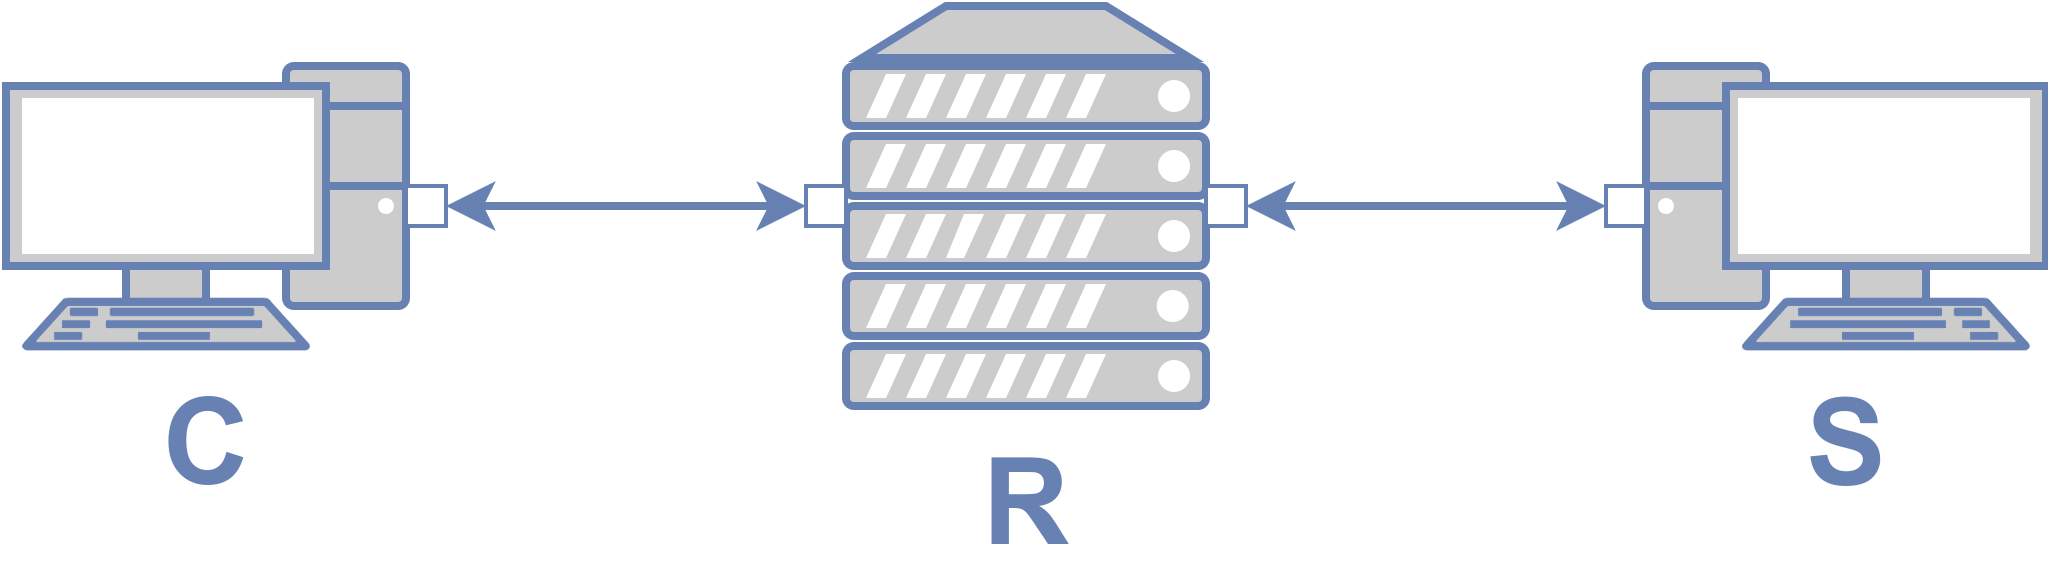
\includegraphics[width=6cm]{figures/testbed.png}
  \end{center}
  \vspace{-0.5cm}
  \caption{
    Performance Measurements Setups. C = Client. S = Server. R = Router/Middlebox.}
  \label{fig:perf_testbed}
    \vspace{-0.5cm}
\end{figure}


The first question that we want to answer is whether \tcpls can compete with the traditionnal \tls over \tcp stack. We then compare our \tcpls prototype with different \quic implementations.


\paragraph*{\tcpls}
For all the \tcpls measurements, we used a custom application that performs large memory-to-memory transfers over a \tcpls session using a single stream. \tcpls was configured to use the \todo{AES-...} encryption scheme.
Fig.~\ref{fig:perf} provides the goodput measured in our testbed. We report both the bandwidth in megabits per second and packets per second.  Each bar in this figure is the average over \todo{x} runs. The bottom bar is the highest goodput that we measured with \tcpls: \todo{12 Gbps}. This result was obtained with jumbo frames (i.e. 9000 bytes MTU) and using TCP Segmentation Offload (TSO) on the NICs. TSO is a standard feature that is enabled by all high-speed NICS. The next bar shows that with TSO and a standard frame size (1500 bytes MTU), the goodput is still \todo{11 Gbps}. These results should be compared with the 22~Gbps that TCP reaches in the same environment using \texttt{iperf} but without any encryption. We measured that \todo{AES-...} peaks at \todo{xx} Gbps when doing in-memory encrytion/decryption on our testbed's servers.

%the
%shows several interesting results. First, while
%offering similar (and more) capabilities than what QUIC is providing today,
%\tcpls is also more than twice faster than the strongest evaluated QUIC
%implementation (quicly) over CPU limited experimentations. We evaluate \tcpls

We then evaluated the impact of adding the \tcpls-level acknowledgements
described in Sec.~\ref{failover} to support failover.
% Thanks to these acknowledgements, \tcpls can support failover.
From a performance viewpoint, they increase the number of control records and the number of system calls. Our prototype currently sends a \tcpls-ack for every 16 received records, or after having received 15 times the maximum \tls payload \todo{OB ne voit pas la différence}, or upon the expiration of \todo{xx msec} timer. Our measurements indicate that with this functionnality, \tcpls reaches \todo{9.5 Gbps}.


\begin{figure}[!t]
  \begin{center}
    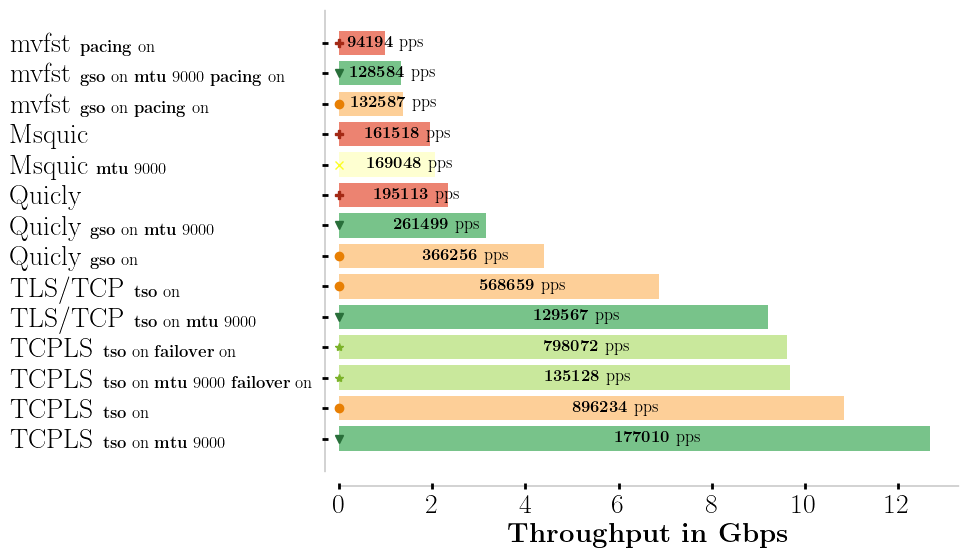
\includegraphics[width=\columnwidth]{figures/perf_analysis.png}
  \end{center}
  \caption{The \tcpls prototype is faster than \tls over \tcp and different \quic implementations.}
  \label{fig:perf}
\end{figure}


%in four different settings: with a path mtu of 1500 or 9000, and with failover
%enabled or not. The failover functionality is an internal stack feature that
%provides session reliability, which increases the number of syscalls that TCPLS
%makes by exchanging TCPLS-level record acknowledgments. We currently send an ac%k
%for
%throughput at the price of a slower recovery in case of network failure.

\paragraph*{\tcpls vs. \tls/\tcp}
We now compare the performance of \tcpls with the traditional \tls over \tcp stack. To have a fair comparison, we use \texttt{picotls}'s client/server
implementation with the same commit as our initial fork for \tcpls.
\todo{test client pour TLS/TCP}
Fig.~\ref{fig:perf} shows that \tls/\tcp provides a lower performance than
\tcpls with regular and jumbo frames. This can be explained by the receiving
buffer size provided to \texttt{read()}, which is hardcoded to 16,384 bytes
\todo{in \texttt{picotls}}. This implementation results in fragmentation on the
receiver and prevents it from using the zero-copy code path provided by the
library. \tcpls uses a larger read buffer and benefits from zero-copy. At first, one may consider this as an unfair comparison, however the devil is in the details. In \tcpls implementation, the application developers cannot touch \texttt{read()}'s interface. This implies that an application developer cannot missuse the relationship between \tls and \tcp by creating fragmented records and doing unecessary copies to handle those fragments. \tcpls's design and implementation try to prevent fragmentation by first, having a sufficiently large read buffer size. Second, \tcpls only starts deciphering a record it has received the entire record. \tls/\tcp record fragmentation is provided by TLS libraries as a usability feature that spares the application developers from taking into account all \tls details, at the cost of lower performance.
With \tcpls application developers can ignore \tls details without missusing the interface, which is the reason why this comparison is interesting.\tcpls constrains the application developer to use the buffer type provided
by the API, but offers zero-copy deciphered records in return.

%\todo{OB: pas sur que la suite est nécessaire} Moreover, but this has not
%yet been implemented, it could be interesting to match the TLS record size to
%the congestion window to deliver faster the data to the application when the
%network is congested.

\paragraph{\tcpls vs. \quic}
Although \quic~\cite{draft-ietf-quic-transport} is a young protocol, there are
already more than a dozen implementations~\cite{marx2020same,quicimplem,yang2020making} under active development. We compiled and installed three representative \quic implementations in our testbed: Facebook's mvfst~\cite{} from Facebook, Microsoft's msquic~\cite{} Fastly's quicly~\cite{}. They are all developed by
large companies that (plan to) use them in production and include their own
benchmarking application to perform throughput measurements. Furhtermore,
mvfast and quicly support Generic Segmentation Offload (GSO), which should improve performance by offloading \udp segmentation and checksum computation available on our NICs. We use the implementation's bechmarking application
as is, exploiting the optional arguments provided by their interface to increase the throughput but drawing the line there. That is, we do not modify the QUIC implementations.

The results shown in Fig.~\ref{fig:perf} show that \tcpls compares favorably
with the tested \quic implementations. The fastest \quic implementation is quicly. Thanks to GSO, it reaches \todo{4 Gbps} in our testbed with a 1500 bytes MTU. This result is directly comparable to \tcpls with TSO enabled,
which still performs more than twice faster at 100\% CPU peak with similar configurations for the transport parameters. Suprisingly, quicly's performance decreases with jumbo frames but is still faster than when GSO is disabled. In our testbed, msquic could only reach \todo{2 Gbps} and mvfst was slower.


%QUIC is young protocol, and all implementations are in active development, with
%different states for their available features and optimizations. For example,
%none of the implementations were able to take advantage of a path mtu larger
%than 1500, and it even degraded the performance in the case of quicly. Two of them
%(quicly and mvfst) have implemented the support for \texttt{gso} leading in the
%case of quicly to more than 4 gb/s of throughput with a udp payload length
%configured to match TCP (1460).


%We perform a throughput evaluation of \tcpls and compare it to several major
%QUIC implementations: mvfst~\cite{} from Facebook, msquic~\cite{} from Microsoft
%and quicly~\cite{} from Fastly. Our choice of QUIC implementations was mainly
%influenced by the availability of a client/server perf tool specifically
%engineered for a throughput evaluation. A second criterion was the advancement
%of the implementation and the quality of the code. We hope to avoid most of the
%bugs negatively impacting their results by selecting the QUIC implementation
%that show advanced features and testings. A third criterion was the development
%language used. \tcpls is written in C, and we prefer to compare it against QUIC
%implementation written in a language compiled by clang or gcc. Mvfst, msquic
%and quicly meet these criteria.


\subsection{Middlebox Interference}

A full evaluation of middlebox interference would require measurements in various operational networks that include such devices \cite{honda2011still,raman2020measuring,o2016tls}. This is outside the scope of this paper and left for further work.
We tested \tcpls against different opensource and commercial stateful
firewalls and proxy implementations and (i.e., pfSense, IPFire, Cisco ASAv, mitmproxy) and found no interference. Still, the security appliances that block
TLS 1.3 or some of its features \cite{lee2019matls,Bock_China,raman2020measuring} would also block \tcpls.
%pervasive monitoring allows for configurable TLS extensions blocking
%\cite{rfc7258}. This is handled properly by \tcpls fallback mechanism.


When faced with middleboxes that intercept TLS 1.3 \cite{Bock_China,raman2020measuring}, we need to consider the two TLS extensions used by \tcpls: \tcpls and \join. If a clients attempts to open a \tcpls session through a \tls termination
proxy, it sends a \textsc{ClientHello} with the \tcpls extension.
If the proxy does not support \tcpls, it replies with a \textsc{ServerHello}
message that does not include the \tcpls extension. From this point, the client
implicitely fallback to \tls, and continues with the handshake.

Certain legacy \tls server implementations are known not to implement the \tls
specification properly and might abort connections when receiving unknown \tls
extensions. Analogous behavior has been observed in overly restrictive stateful
firewalls. To ensure connectivity in the presence of such policies, \tcpls
implements an explicit fallback mechanism. If a client receives a \tcp \rst in
response to the \tcpls-setup \textsc{ClientHello}, or no response, it
tries negotiating a second non-\tcpls \tls connection, either
immediately or after a timeout. Similarly, a \tcpls \join extension might be
blocked on a path. In this case, the subflow attachment is canceled, and
the application is directly notified to be able to react appropriatly (e.g.,
to cancel a migration attempt).

%We tested \tcpls against opensource and commercial stateful firewalls and proxy
%implementations and (i.e., pfSense, IPFire, Cisco ASAv, mitmproxy) and found no
%interferences. Still, certain middlebox security appliances that implement
%pervasive monitoring allows for configurable TLS extensions blocking
%\cite{rfc7258}. This is handled properly by \tcpls fallback mechanism.


\subsection{Bandwidth Aggregation}

We compare the capability of \tcpls to the state of the art \mptcp. Both
protocols run in the same Mininet topology with two IP paths available, each
offering 25 mbps and a latency of 10 ms. The experiment consists to transfering
a file over a single path and then enabling the second one at $5$ seconds. For
\mptcp, the new path is detected after we up the client's second interface. For
\tcpls, managing paths is easier: the application can use the API to add local
or peer-related addresses at any point of the connection. In that case, we add
the information at $5$ seconds, connect to the peer and attach a new stream to
this new connection. Our results are displayed in
Figure~\ref{fig:multipath_aggregation}. Both stacks enable the aggregation of the
goodput to ~50 mbps. There are two major differences displayed by the stacks.
First, upping the interface, adding the routes and detecting the new path in
the case of \mptcp is time consuming. It leads \mptcp to react slower than
\tcpls regarding the availability of the new path. Second, \tcpls's aggregated
goodput seems less stable than \mptcp. This discrepency is explained by the
difference of chunk size manipulated by the reordering algorithm: \mptcp
reorders packets with a payload of $1,460$ bytes, while \tcpls is this experiment
reorders records with the maximum payload size of $16,384$ bytes. That means
that \tcpls, upon unordered records, would need to reorder and deliver much
larger chunks of data, leading to larger goodput irregularities than \mptcp.
However, \tcpls might  negotiate the record size to smooth out this
irregularity. Setting a record size around $1,500$ bytes would make them lookalike,
but would be more CPU costly.

\begin{figure}[!t]
  \begin{center}
    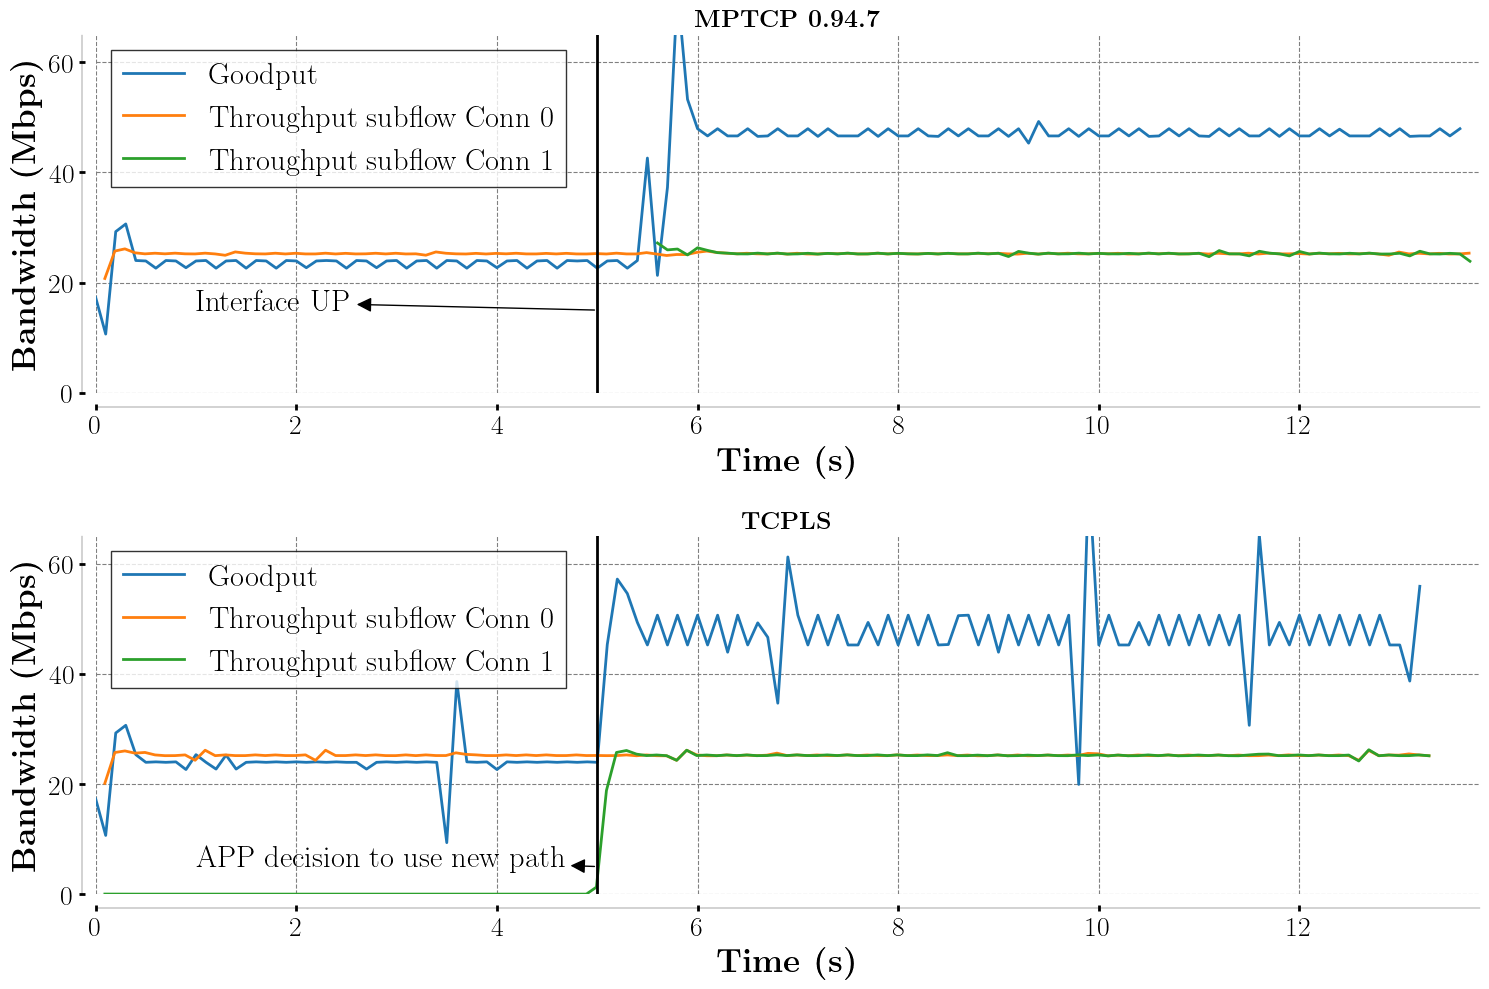
\includegraphics[width=\columnwidth]{figures/aggregate_dual.png}
  \end{center} 
  \caption{Bandwidth aggregation comparison between \mptcp and
    \tcpls.}
  \label{fig:multipath_aggregation}
\end{figure}

\subsection{Application-Level Migration}


Detailler pourquoi on a besoin du controle applicatif pour la migration, et à
quels cas du monde réels ils s'appliquent


Fig.~\ref{fig:conn_migration} shows the result of an Application-level
connection migration demo using the API (i.e., it is left to the
application to decide when to migrate, and we expose a simplistic code flow to
perform it). In this experiment, we use an IPMininet network~\cite{ipmininet, jadin2020educational} \todo{BD: Mininet above, IPMininet here with different refs.  Make sure to be consistent}
composed of a client and a server, both dual-stacks. One path within the
network is composed of OSPF routers with IPv4 only, and one path is composed of
OSPF6 routers IPv6 only. We configure the bandwidth to 30Mbps, the lowest delay
to the v4 link. Our application downloads a 60 MB file from a server and migrates to the v6 connection in the middle of the download.

Triggering the connection migration involves chaining 5 API calls:
first, \texttt{tcpls\_handshake()} configured with handshake properties announcing a \join over the v6 connection id. Then, the creation of a new stream
\texttt{tcpls\_stream\_new()} for the v6 connection id, finally followed by the attachment of this new stream \texttt{tcpls\_streams\_attach()} and the secure closing of the v4 \tcp connection using \texttt{tcpls\_stream\_close()}. Following these events, the server seamlessly switches the path while looping over \texttt{tcpls\_send} to send the file content. Note that all the events trigger callbacks on the server side, to let the server react appropriately if other requirements need to be fulfilled.

\tcpls's application connection migration takes advantage of multipath to offer
a smooth handover to applications, which \tcpls cannot do at the moment.

\begin{figure}[!t]
  \centering
  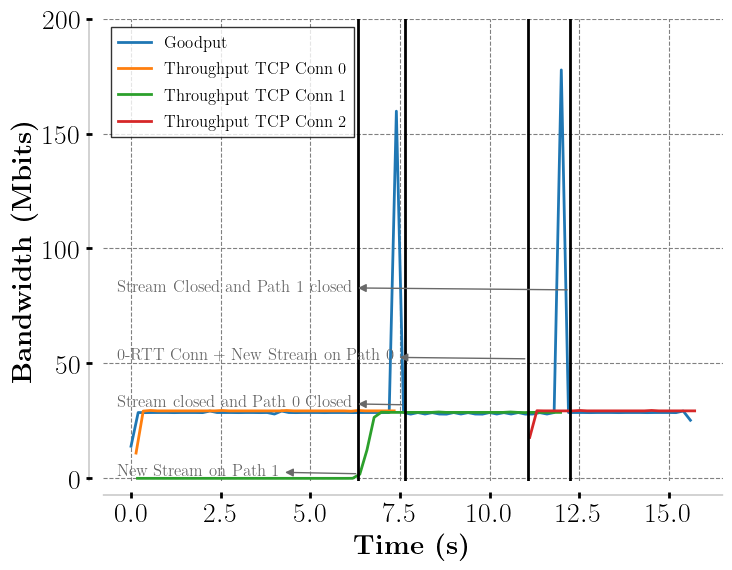
\includegraphics[width=\columnwidth]{figures/migration.png}
  \caption{Application-level connection migration during a 60MB file download.}
  \label{fig:conn_migration}
\end{figure}

\subsection{Failover}

1) analyse du temps de recovery pour different type de cassure, et comparaison avec mptcp
2) discuter une propriété de "connection reliability" => ca casse, on restabilise le plus vite possible
3) montrer que le path manager est important pour cette propriété, et que ce n'est pas encore au point pour mptcp, mpquic, etc

Mptcp overhead: 1.0744997978210449
TCPLS overhead: 1.0994282363439873
MPTCP overhead/TCPLS overhead:              0.9773259975513828


\begin{figure}[!t]
  \begin{center}
    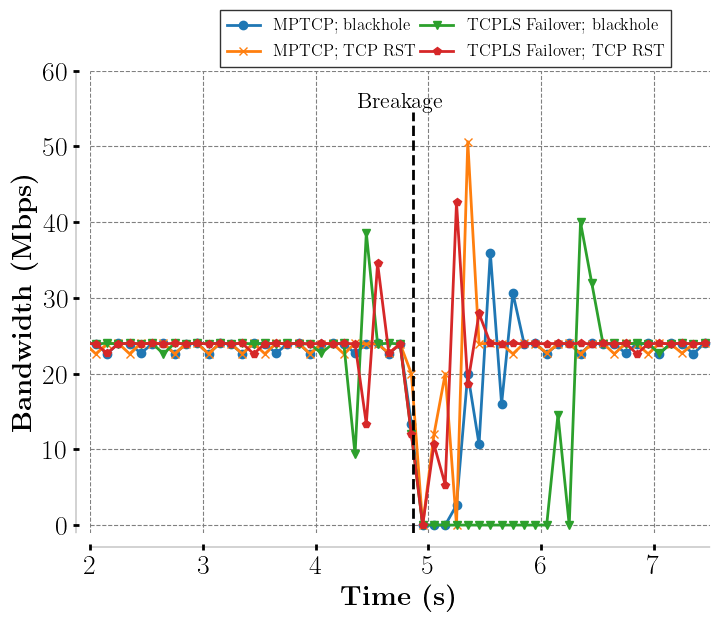
\includegraphics[width=\columnwidth]{figures/breakage_analysis.png}
  \end{center}
  \caption{Recovery speed analysis.}
\end{figure}


\begin{figure}[!t]
  \begin{center}
    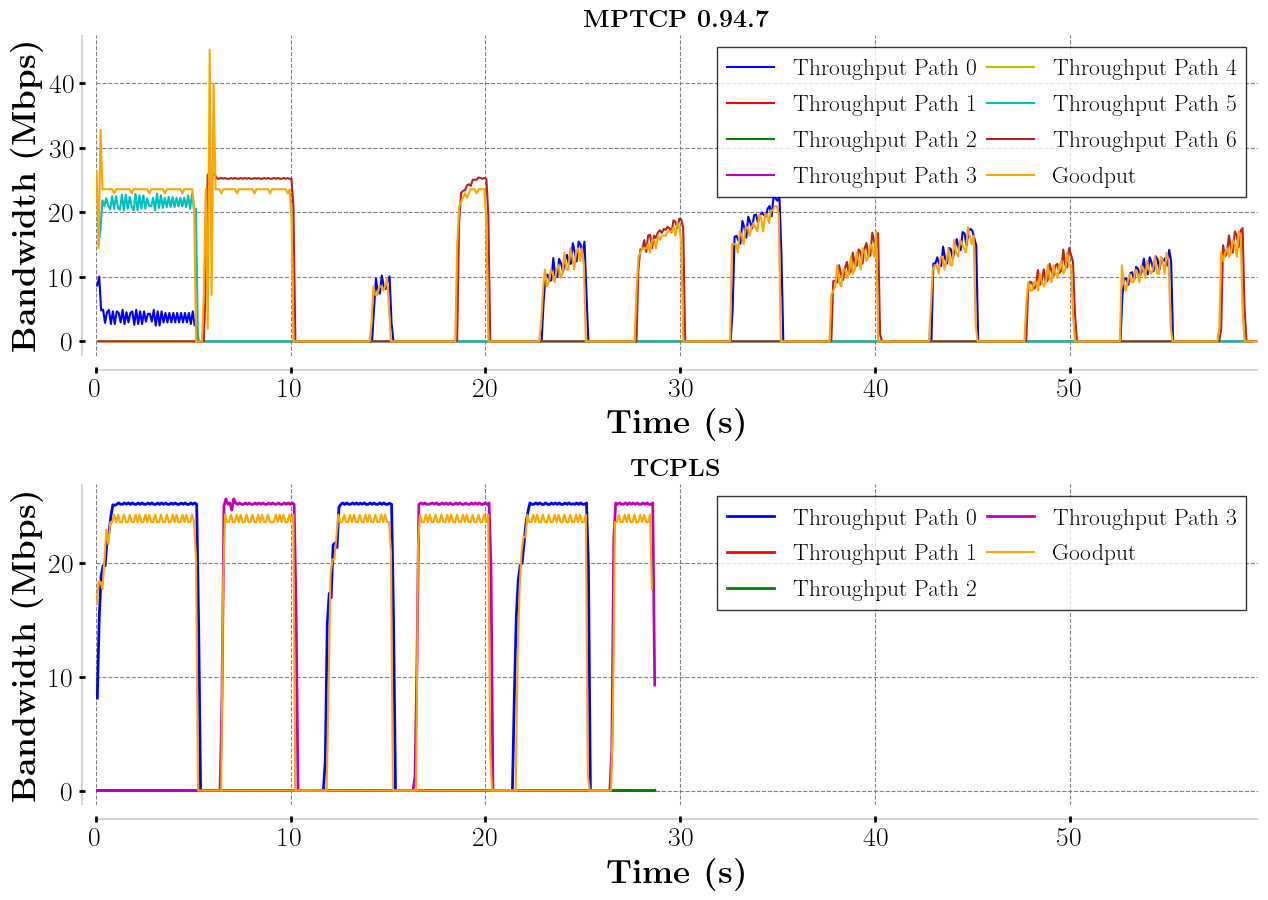
\includegraphics[width=\columnwidth]{figures/tcpls_mptcp.png}
  \end{center}
  \caption{Connection reliability: influence of the path manager and congestion
  control.}
\end{figure}



\subsection{Dynamically Extending \tcpls}

The \tcpls streams enable new use case. Obviously, a \tcpls application can
create and use different streams to carry data. However, since these streams
are generic, they can also be used by the \tcpls implementation itself to
exchange control information. To demonstrate the versatily of these control
streams, we extended \tcpls to enable a server to push a different congestion
control scheme to a specific client over an existing \tcpls session. Recent
work on restructuring congestion control has proposed a generic architecture
for congestion controllers \cite{narayan2018restructuring}.
During the last years, the Linux kernel developpers have relied on eBPF
to make the Linux TCP/IP stack \cite{brakmo2017tcp,tran2020beyond} easier
to extend. Since Linux kernel version 5.6, an application can inject
a different congestion control scheme entirely implemented using eBPF. A similar
approach was proposed in Pluginizing \quic~\cite{de2019pluginizing}.  We
leverage these new eBPF capabilities to demonstrate the feasibility of injecting
and updating a congestion control scheme during a \tcpls session.

We perform our experiment using Mininet \todo{BD: same remark as above.  Mininet
  or IPMininet} over a 100 Mbps emulated link that has a 60 msec delay.
Fig.~\ref{fig:vegasCubic} shows a client that uses the TCP
Vegas~\cite{10.1145/190314.190317} congestion control scheme to upload a file.
This \tcpls session fully uses the bottleneck link. After some time, another
client starts an upload, but using the CUBIC congestion
controller~\cite{rfc8312}. This results in an unfair distribution of the
bandwidth. The server then sends the eBPF bytecode of the CUBIC congestion
control scheme to the \tcp Vegas client that injects it in its kernel and the
unfairness disappears.  We performed the same experiment for different delay,
varying from 10ms to 100ms.

\begin{figure}[!t]
  \begin{center}
    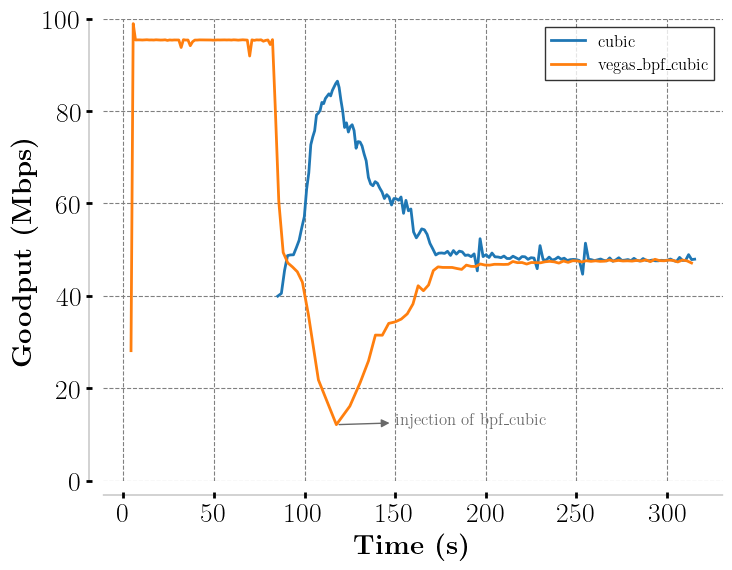
\includegraphics[width=6cm]{pretty_plotify/plots/vegas_cubic.png}
  \end{center}
  \caption{\tcpls hosts can exchange congestion control schemes and activate them during a \tcpls session.}
  \label{fig:vegasCubic}
\end{figure}
